\subsection{Zoom}

The last alteration analyzed is the zoom. \Fig~\ref{fig:acc_zo_wu} illustrates how the accuracy changes with altered data by the zoom. The accuracy of both networks starts to decrease as soon as the zoom level is increased, suggesting a poor robustness to this alteration.

The last alteration under examination is the zoom. In \Fig~\ref{fig:acc_zo_wu}, it is possible to observe how the accuracy is affected by varying levels of zoom. Notably, as the zoom level increases, the accuracy of both networks begins to decline, indicating a lack of robustness against this alteration.

\begin{figure}[h]
	\centering
	\begin{subfigure}{.5\textwidth}
		\centering
		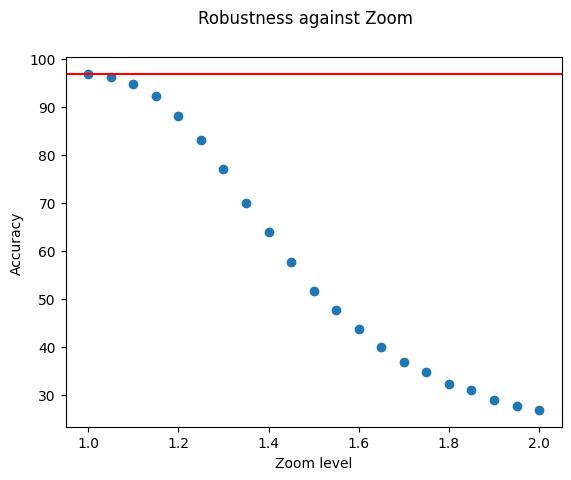
\includegraphics[width=0.9\linewidth]{ImageFiles/EvalBNN/ZO/WU/acc}
		\caption{BNN}
		\label{fig:zo_acc_wu_bnn}
	\end{subfigure}%
	\begin{subfigure}{.5\textwidth}
		\centering
		us		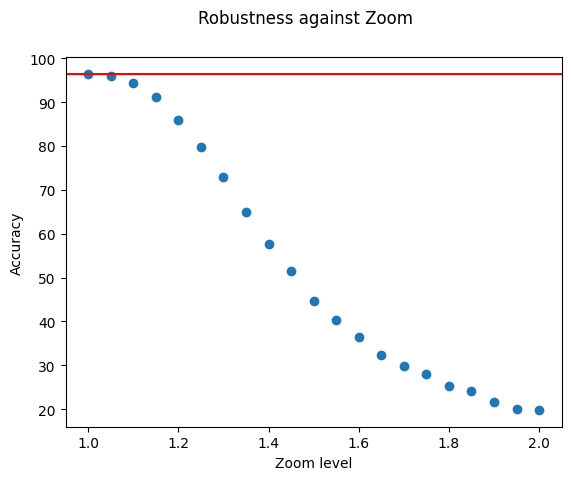
\includegraphics[width=0.9\linewidth]{ImageFiles/EvalANN/zoom_ann}
		\caption{Standard NN}
		\label{fig:zoom_ann}
	\end{subfigure}
	\caption{Accuracy trend for zoom}
	\label{fig:acc_zo_wu}
\end{figure}

The poor robustness is confirmed by the quantitative metrics computed, which are $0.7731$ for the BNN and $0.7467$ for the standard NN.

The uncertainties estimated by the BNN exhibit a defined pattern in this case, as depicted in \Fig~\ref{fig:zo_uncertainty}. Specifically, the aleatoric uncertainty, shown in \Fig~\ref{fig:zo_aleatoric}, follows an exponential trend, reaching a saturation level around a zoom level of $1.4$. On the other hand, epistemic uncertainty, illustrated in \Fig~\ref{fig:zo_epistemic}, reflects the trend of accuracy. In essence, as the zoom level increases, the network becomes progressively less confident in its predictions.

\begin{figure}[h]
	\centering
	\begin{subfigure}{.5\textwidth}
		\centering
		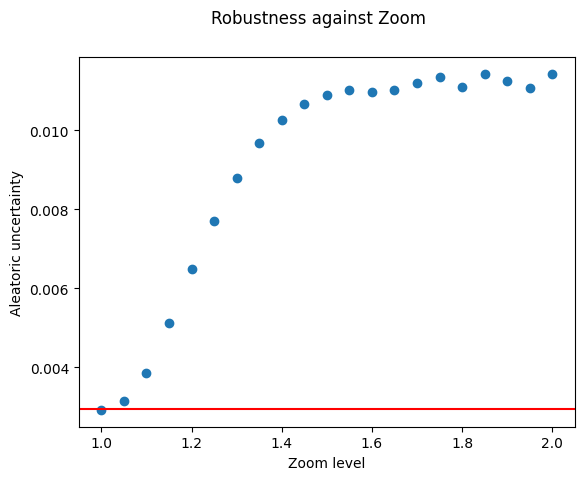
\includegraphics[width=0.9\linewidth]{ImageFiles/EvalBNN/ZO/aleatoric}
		\caption{Aleatoric uncertainty}
		\label{fig:zo_aleatoric}
	\end{subfigure}%
	\begin{subfigure}{.5\textwidth}
		\centering
		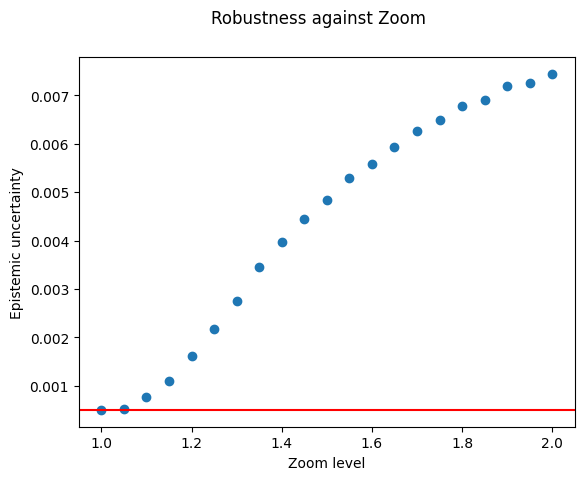
\includegraphics[width=0.9\linewidth]{ImageFiles/EvalBNN/ZO/epistemic}
		\caption{Epistemic uncertainty}
		\label{fig:zo_epistemic}
	\end{subfigure}
	\caption{Uncertainty trend for zoom}
	\label{fig:zo_uncertainty}
\end{figure}

\vspace{0.3cm}
\textbf{Classification using aleatoric uncertainty}
\vspace{0.1cm}

\todo{wating loading}

\begin{figure}[h]
	\centering
	\begin{subfigure}{.33\textwidth}
		\centering
		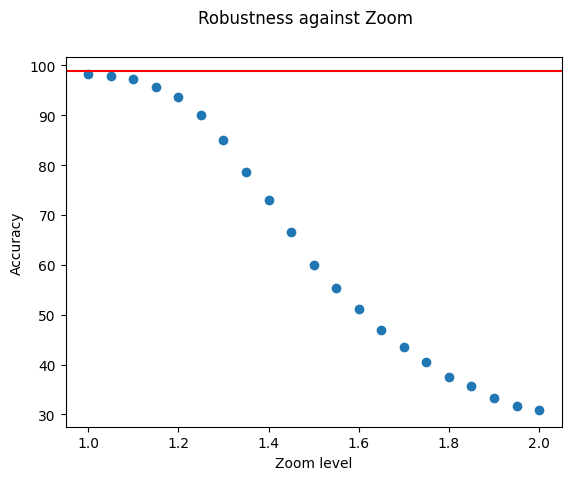
\includegraphics[width=0.9\linewidth]{ImageFiles/EvalBNN/ZO/AU/acc}
		\caption{Accuracy using aleatoric \\ uncertainty}
		\label{fig:zo_au_acc}
	\end{subfigure}%
	\begin{subfigure}{.33\textwidth}
		\centering
		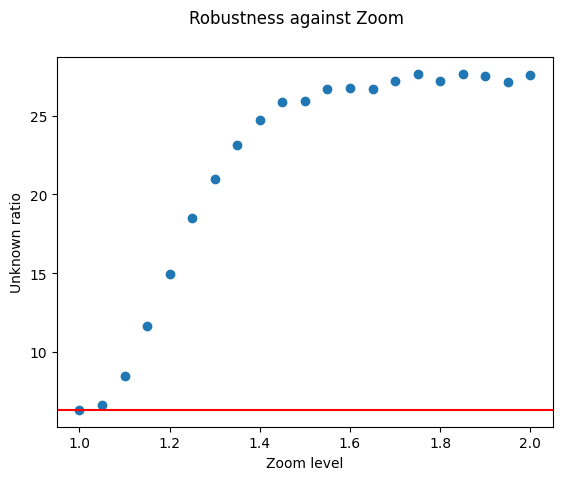
\includegraphics[width=0.9\linewidth]{ImageFiles/EvalBNN/ZO/AU/unkn}
		\caption{Unknown ratio using aleatoric uncertainty}
		\label{fig:zo_au_unkn}
	\end{subfigure}%
	\begin{subfigure}{.33\textwidth}
		\centering
		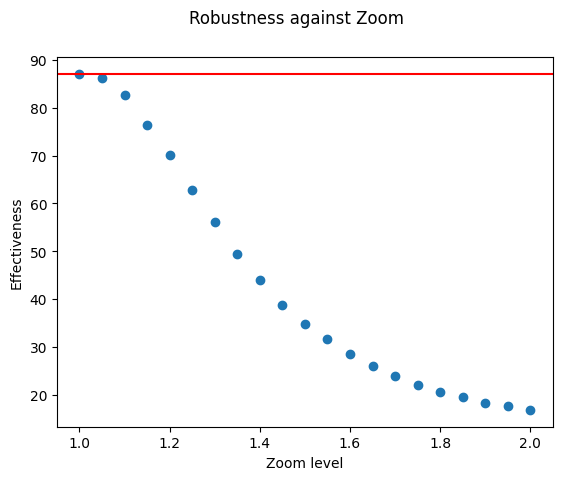
\includegraphics[width=0.9\linewidth]{ImageFiles/EvalBNN/ZO/AU/eff}
		\caption{Effectiveness using aleatoric uncertainty}
		\label{fig:zo_au_eff}
	\end{subfigure}
	\caption{Robustness graph for zoom when aleatoric uncertainty is employed in the classification}
	\label{fig:zo_au}
\end{figure}

\Tab~\ref{table:rob_zo_au} presents the quantitative robustness measurements.
\begin{table}[h]
	\centering
	\begin{tabular}{|| l | l ||} 
		\hline
		\textbf{Parameter} & \textbf{Value} \\
		\hline
		\hline
		$rob_{Zoom}$ & $0.7974$ \\
		$robInd_{Zoom}$ & $0.8667$ \\
		$robAug_{Zoom}$ & $0.7124$ \\	
		\hline
	\end{tabular}	
	\caption{Robustness metrics for zoom when the aleatoric uncertainty is employed}
	\label{table:rob_zo_au}
\end{table}

\vspace{0.3cm}
\textbf{Classification using epistemic uncertainty}
\vspace{0.1cm}

The outcomes obtained using epistemic uncertainty are displayed in \Fig~\ref{fig:zo_au}. An important observation relates to the unknown ratio, depicted in \Fig~\ref{fig:zo_au_unkn}, which reaches values of approximately $40\%$. This implies that roughly half of the predictions are classified as unknown. However, despite this, the accuracy, shown in \Fig~\ref{fig:zo_au_acc}, does not exhibit any improvement. This underscores, once again, the ineffectiveness of epistemic uncertainty in identifying uncertain situations and enhancing robustness.

\begin{figure}[h]
	\centering
	\begin{subfigure}{.33\textwidth}
		\centering
		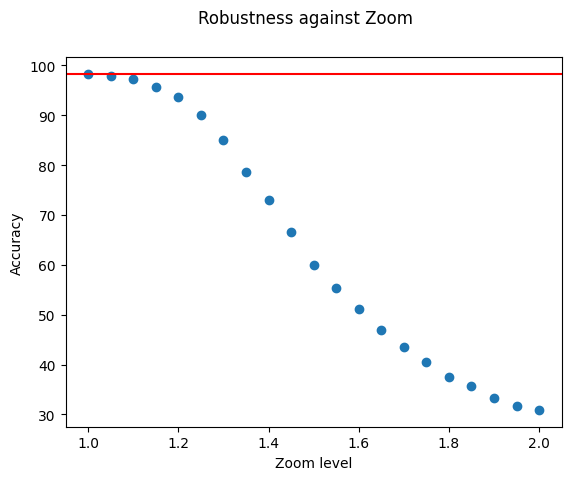
\includegraphics[width=0.9\linewidth]{ImageFiles/EvalBNN/ZO/EU/acc}
		\caption{Accuracy using epistemic \\ uncertainty}
		\label{fig:zo_eu_acc}
	\end{subfigure}%
	\begin{subfigure}{.33\textwidth}
		\centering
		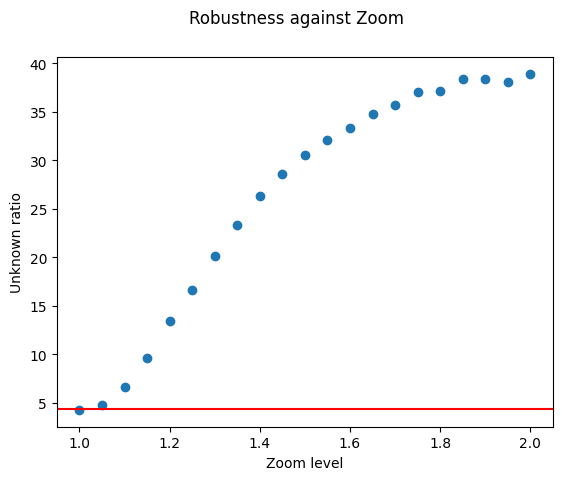
\includegraphics[width=0.9\linewidth]{ImageFiles/EvalBNN/ZO/EU/unkn}
		\caption{Unknown ratio using \\ epistemic uncertainty}
		\label{fig:zo_eu_unkn}
	\end{subfigure}%
	\begin{subfigure}{.33\textwidth}
		\centering
		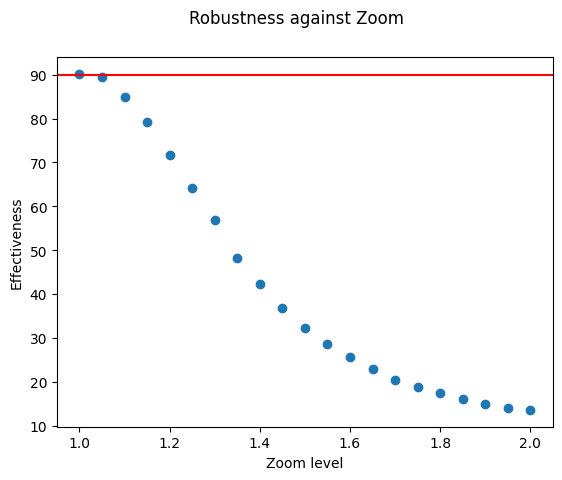
\includegraphics[width=0.9\linewidth]{ImageFiles/EvalBNN/ZO/EU/eff}
		\caption{Effectiveness using \\ epistemic uncertainty}
		\label{fig:zo_eu_eff}
	\end{subfigure}
	\caption{Robustness graph for zoom when epistemic uncertainty is employed in the classification}
	\label{fig:zo_eu}
\end{figure}

\Tab~\ref{table:rob_zo_eu} displays the robustness metrics.

\begin{table}[h]
	\centering
	\begin{tabular}{|| l | l ||} 
		\hline
		\textbf{Parameter} & \textbf{Value} \\
		\hline
		\hline
		$rob_{Zoom}$ & $0.7991$ \\
		$robInd_{Zoom}$ & $0.8598$ \\
		$robAug_{Zoom}$ & $0.7060$ \\	
		\hline
	\end{tabular}	
	\caption{Robustness metrics for zoom alteration when the epistemic uncertainty is employed}
	\label{table:rob_zo_eu}
\end{table}

\vspace{0.3cm}
\textbf{Classification using standard deviation}
\vspace{0.1cm}

The results obtained when using standard deviation, as illustrated in \Fig~\ref{fig:zo_vu}, exhibit the same behavior as when using aleatoric uncertainty.

\begin{figure}[h]
	\centering
	\begin{subfigure}{.33\textwidth}
		\centering
		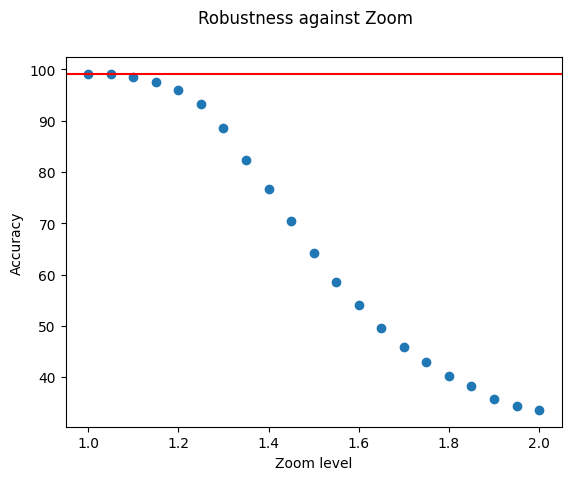
\includegraphics[width=0.9\linewidth]{ImageFiles/EvalBNN/ZO/VU/acc}
		\caption{Accuracy using standard \\ deviation}
		\label{fig:zo_vu_acc}
	\end{subfigure}%
	\begin{subfigure}{.33\textwidth}
		\centering
		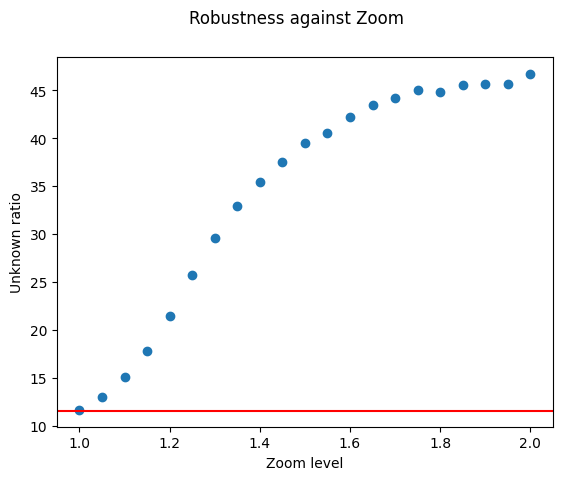
\includegraphics[width=0.9\linewidth]{ImageFiles/EvalBNN/ZO/VU/unkn}
		\caption{Unknown ratio using \\ standard deviation}
		\label{fig:co_vu_unkn}
	\end{subfigure}%
	\begin{subfigure}{.33\textwidth}
		\centering
		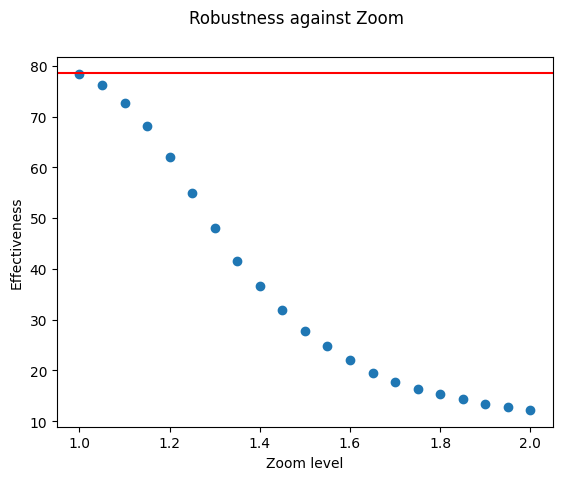
\includegraphics[width=0.9\linewidth]{ImageFiles/EvalBNN/ZO/VU/eff}
		\caption{Effectiveness using standard deviation}
		\label{fig:zo_vu_eff}
	\end{subfigure}
	\caption{Robustness graph for zoom when standard deviation is employed in the classification}
	\label{fig:zo_vu}
\end{figure}

\Tab~\ref{table:rob_zo_vu} gives the quantitative robustness measurements.

\begin{table}[h]
	\centering
	\begin{tabular}{|| l | l ||} 
		\hline
		\textbf{Parameter} & \textbf{Value} \\
		\hline
		\hline
		$rob_{Zoom}$ & $0.8102$ \\
		$robInd_{Zoom}$ & $0.8432$ \\
		$robAug_{Zoom}$ & $0.7032$ \\	
		\hline
	\end{tabular}	
	\caption{Robustness metrics for zoom when the standard deviation is employed}
	\label{table:rob_zo_vu}
\end{table}

\vspace{0.3cm}
\textbf{Comparison}
\vspace{0.1cm}

Table~\ref{table:rob_zo} presents a comparison of the computed metrics. It is evident that the network lacks robustness for any uncertainty type. In this scenario, a possible solution could be to change the network architecture or employ techniques for improving robustness, such as \textit{data augmentation}. Additionally, revising the alteration range and conducting another domain analysis may also be beneficial as the robustness is defined with respect to an alteration range.

\begin{table}[h]
	\centering
	\begin{tabular}{|| l | l | l | l ||} 
		\hline
		\textbf{Parameter} & \textbf{Aleatoric} & \textbf{Epistemic} & \textbf{Standard deviation} \\
		\hline
		\hline
		$rob_{Zoom}$ & $0.7974$ & $0.7991$ & $0.8102$ \\
		$robInd_{Zoom}$ & $0.8667$ & $0.8598$ & $0.8432$ \\
		$robAug_{Zoom}$ & $0.7125$ & $0.7060$ & $0.7032$ \\	
		\hline
	\end{tabular}	
	\caption{Summary of the robustness metrics for zoom}
	\label{table:rob_zo}
\end{table}